\section{Implementation}
\label{sec:implementation}

I implemented a Two-Layer Neural Net with Sofmax Classifier.
The network consists of an input layer, a hidden layer with ReLU activation, and an output layer with softmax.
We trained the model using stochastic gradient descent (SGD), and the gradients were derived analytically and verified with numerical gradient checking.

\textbf{Forward Pass.} The forward pass computes activations in two stages. The first layer computes $z_1 = XW_1 + b_1$, followed by ReLU activation $a_1 = \max(0, z_1)$. The second layer computes the final class scores as $scores = a_1W_2 + b_2$.

\textbf{Loss Computation.} We used the softmax loss function with L2 regularization. To ensure numerical stability, logits were shifted before computing softmax probabilities.

\textbf{Backward Pass.} Gradients of all parameters ($W_1, b_1, W_2, b_2$) were derived analytically using backpropagation and validated through numerical gradient checking.

\textbf{Training.} Training was done using mini-batch Stochastic Gradient Descent (SGD). Each epoch involved computing gradients on a random subset of the data, updating parameters using the gradients, and decaying the learning rate. Training and validation accuracy were monitored every epoch to detect overfitting or underfitting.

\textbf{Prediction.} The final prediction was made by computing class scores and selecting the index with the highest score using \texttt{argmax}.


\section{Results}
\label{sec:results}

The model was trained and evaluated on the MNIST dataset.
With tuned hyperparameters, our best model achieved a validation accuracy of 92.5\% and test accuracy of 90.88\%.

\textbf{Best Configuration:} 
\begin{itemize}
  \item Learning rate: 0.1
  \item Hidden layer size: 200
  \item Regularization strength: 0.0001
  \item Batch size: 200
  \item Num iters: 1000
  \item Learning rate decay: 0.95
\end{itemize}

\begin{figure}[h]
\centering
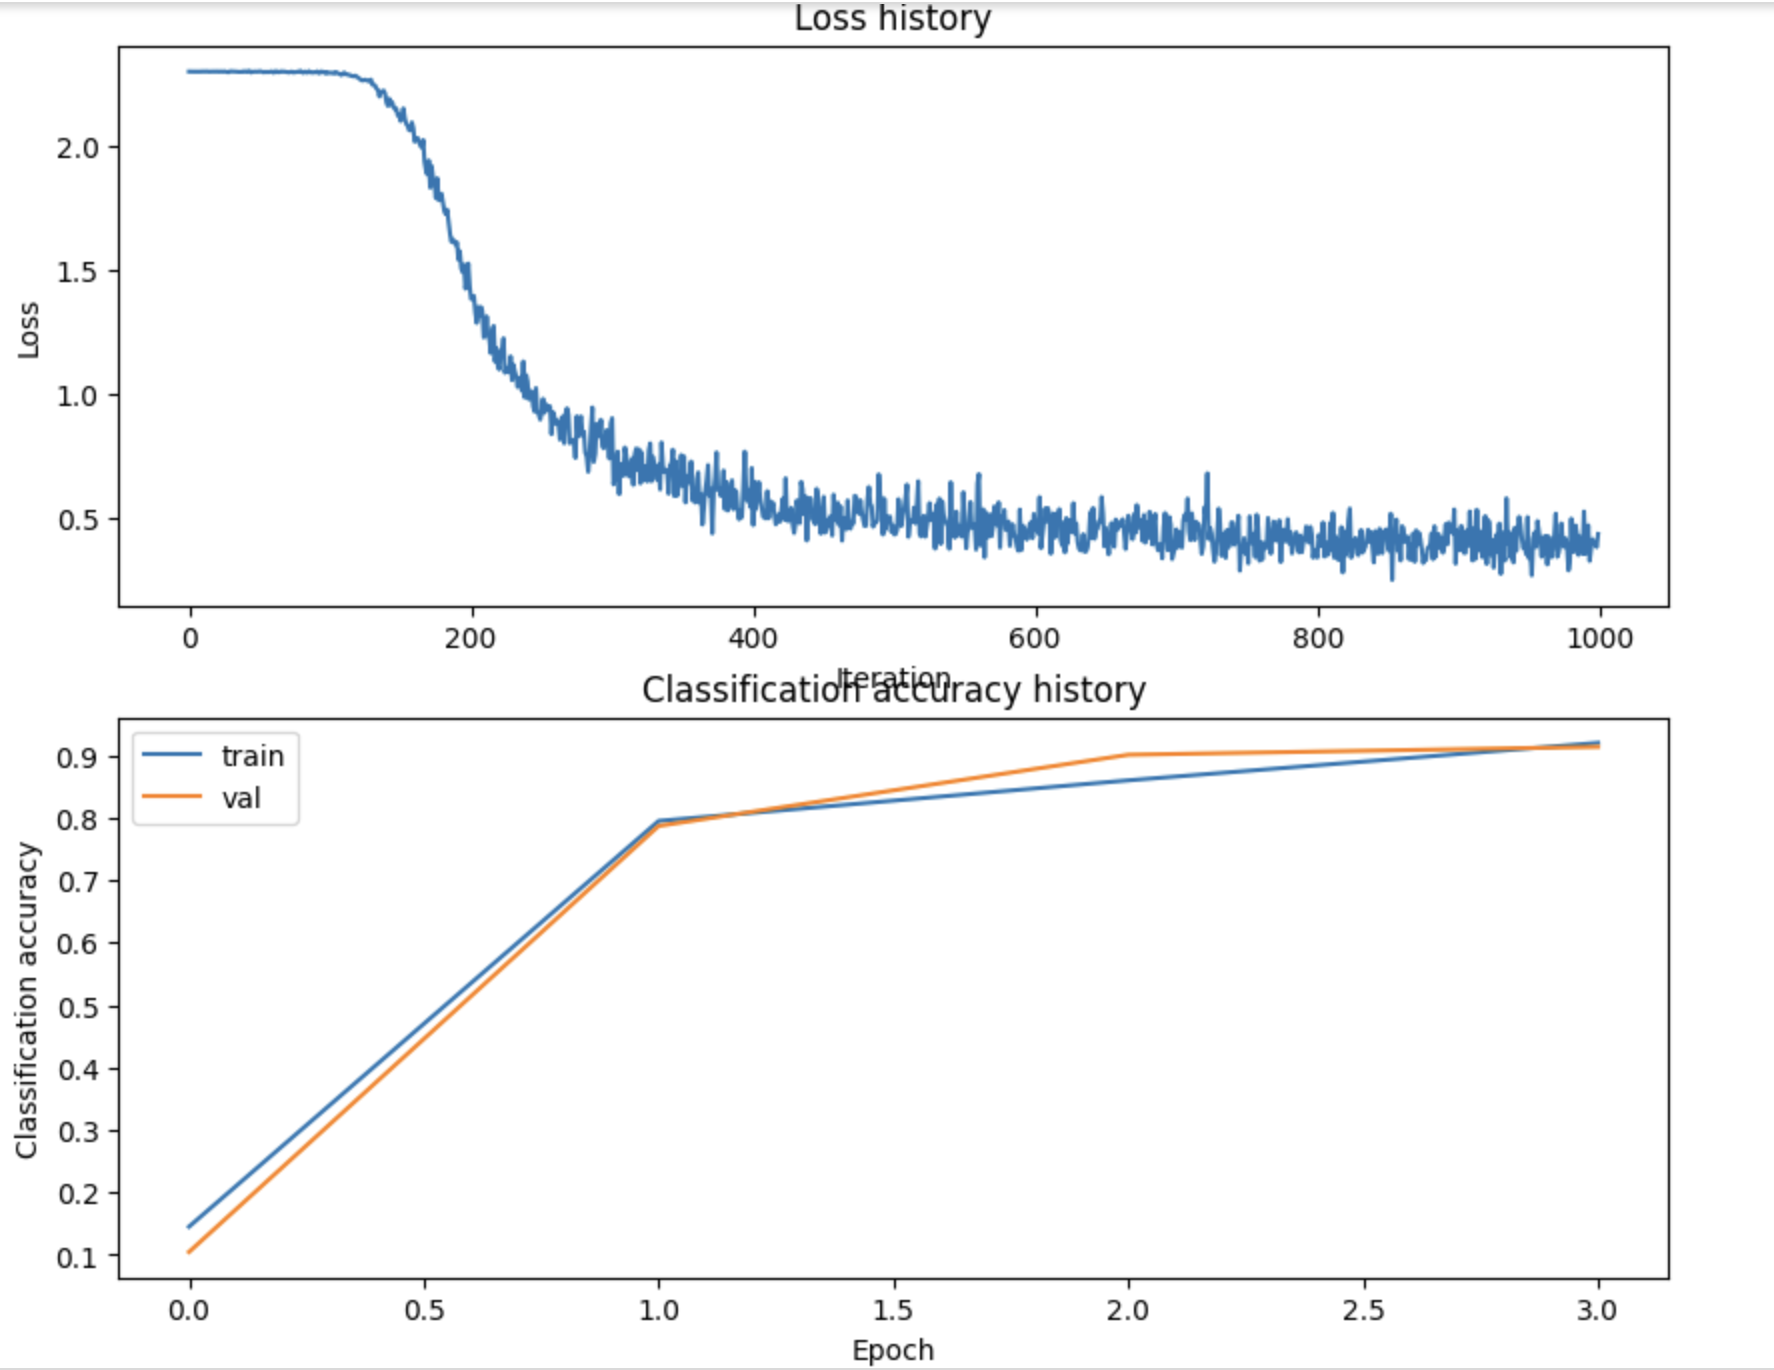
\includegraphics[width=0.8\linewidth]{loss_accuracy.png}
\caption{Loss history and Classification accuracy history}
\end{figure}

\begin{figure}[h]
\centering
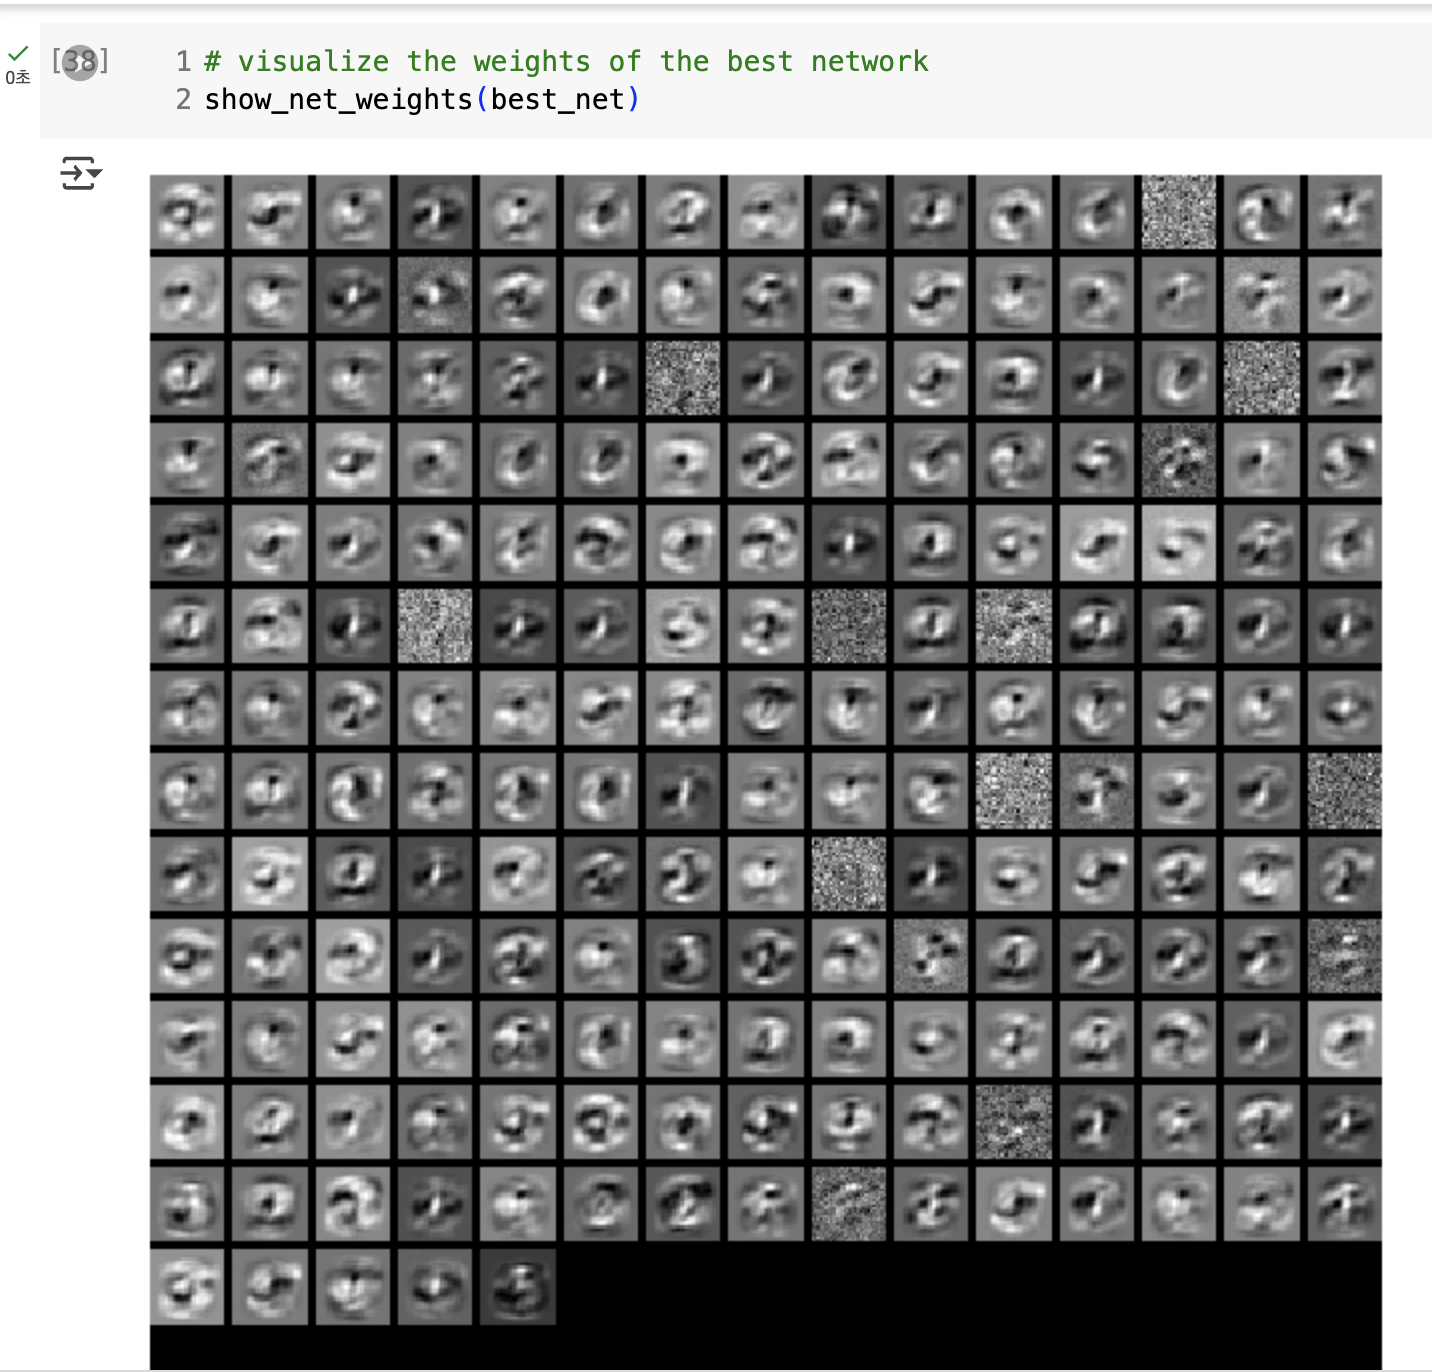
\includegraphics[width=0.8\linewidth]{show_net_weights.png}
\caption{Visualize the weights of the network}
\end{figure}

\begin{figure}[h]
\centering
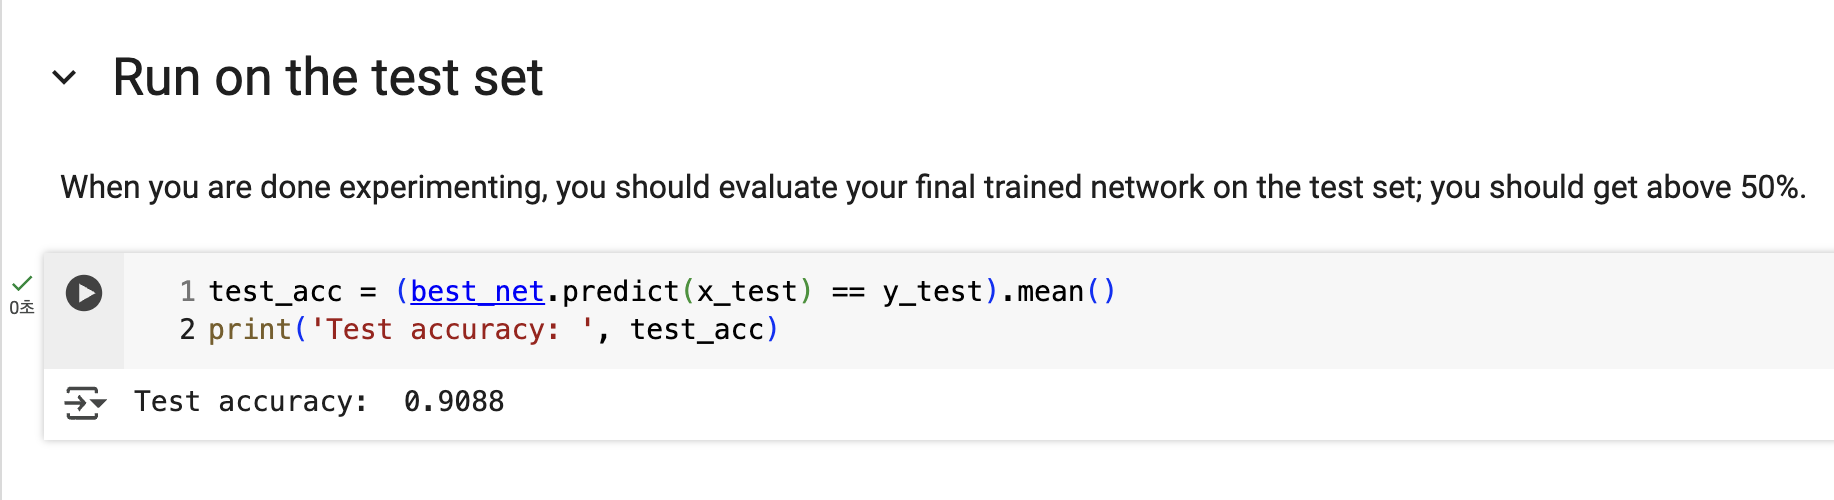
\includegraphics[width=0.8\linewidth]{test_accuracy.png}
\caption{Final test accuracy of 90.88\% achieved on the MNIST dataset.}
\end{figure}

\section{Discussion}
\label{sec:discussion}

The learning rate had a significant impact on convergence.
Small learning rates led to slow training, while large rates caused unstable updates.
We found that using a learning rate around $10^{-1}$ with regularization strength $10^{-3}$ gave the best results.

The hidden layer size also affected the model capacity. Larger hidden sizes increased accuracy but led to overfitting.
The validation accuracy tracked training accuracy well, indicating the model generalized properly with the chosen settings.

Our final model surpassed the target validation accuracy of 36\%, achieving over 90\%.
